\subsection{Braided Monoidal Structure}

As we have already seen for symmetric monoidal categories, they are an example of
colored symmetric operads and can be defined using an op-fibration over $\Fin$ that satisfies
the Segal condition. In this section, we will define representable colorad braided operad and as it turns
out they will be colored braided operads that correspond to braided monoidal categories.
Later, we then see that there is again a forgetful functor that is an op-fibration and fullfills 
the Segal condition.

\begin{defin}
    Let $\B$ be a colored braided operad. We call $\B$ representable if it fullfills the following:
    Let $I$ be a finite set and $\widetilde{I}$ an $I$-labeled configuration. 
    For any collection of colors $\{X_i\}_{i \in I}$ there is a color
    $$\bigotimes_{i \in \widetilde{I}} X_i$$
    such that for every 
    $$f \in \Mul_{\B}^{\widetilde{I}}\left(\left\{X_i\right\}_{i \in I}, \bigotimes_{i \in \widetilde{I}} X_i\right)$$
    the following universal property holds:
    Let $Y$ be a color in $\B$. Then for all $I$-labeled configurations $\widetilde{I}'$ and 
    $g \in \Mul_{\B}^{\widetilde{I}'}(\{X_i\}_{i \in I}, Y)$ there exists a unique

    $$\bar{g} \in \Mul_{\B}^{\id^1}\left(\left\{\bigotimes_{i \in \widetilde{I}} X_i\right\}, Y\right)$$

    such that for a composition map $\gamma$ corresponding to any path $\eta$:
    \begin{center}
        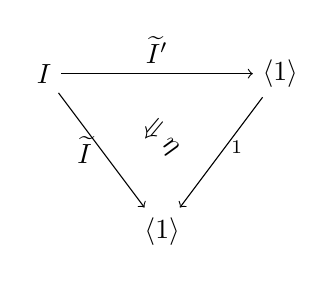
\begin{tikzpicture}
            % Define node positions
            \node (B) at (0, 2) {$I$};
            \node (C) at (3, 2) {$\langle 1 \rangle$};
            \node (A) at (1.5, 0) {$\langle 1 \rangle$};
            
            % Draw arrows
            \draw[->] (B) -- (C) node[midway, above] {$\widetilde{I}'$};
            \draw[->] (B) -- (A) node[midway, left] {$\widetilde{I}$};
            \draw[->] (C) -- (A) node[midway, right] {$\id^1$};
            
            % Natural transformation arrow
            \node[rotate=-40] at (1.5, 1.2) {$\Downarrow \eta$};
            % \node at (1.7, 1.2) {$\eta$};
        \end{tikzpicture}
    \end{center}
    we have:
    \[
        g = \gamma(f, \bar{g})
    \]
\end{defin}

We want to see in this section that this definition yields a
braided monoidal structure on the underlying
category of a colored braided operad $\B$.

\begin{const}\label{con:braidmon}
    Let $\B$ be a representable colored braided operad. 
    We denote the underlying category by $\C$.
    We define
    \[
        \otimes \colon \C \times \C \to \C
    \]
    to be the functor that maps
    \[
        (X_1,X_2) \mapsto \bigotimes_{i \in b_2} X_i
    \]
    where $b_2$ denotes the basepoint configuration in $\E_2(2)$ being 
    a $\langle 2 \rangle^{\circ}$-configuration.




    Let $\beta$ denote the following morphism in $\Br$
     \begin{align*}
         \beta \colon \langle 2 \rangle &\to \langle 2 \rangle \\
         1 &\mapsto 2 \\
         2 &\mapsto 1 \\
     \end{align*}
with the trivial collection $(\id^2, \id^1)$.
Further, let 
\begin{align*}
    \mu \colon \langle 2 \rangle &\to \langle 1 \rangle \\
    1 &\mapsto 1 \\
    2 &\mapsto 1 \\
\end{align*}
be the morphism with the basepoint configuration $b_2 \in \E_2(2)$:
\begin{center}
    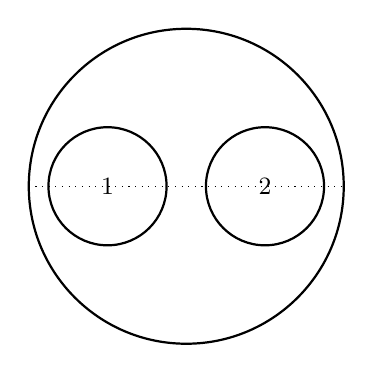
\begin{tikzpicture}
                        % First element (left)
                        \node at (1, 0) {\small $2$};
                        \node at (-1, 0) {\small $1$};
                        
                        \draw[thick] (0,0) circle (2);
                        \draw[thick] (1, 0) circle (0.75);
                        \draw[thick] (-1, 0) circle (0.75);
                        \draw[dotted](-2, 0)--(2, 0);       
        \end{tikzpicture}
\end{center}

Since $\pi$ satisfies the op-fibration condition (M1) and the Segal condition (M2), we have that for any $(A,B) \in \C^2 \cong \Cotimes_{\langle 2 \rangle}$ 
there is a cocartesian lift $(A,B) \to A \otimes B$. The cocartesian property ensures that the choice is 
unique up to unique isomorphism.
So, we obtain a well-defined functor
\[
    \otimes \colon \C^2 \to \C.
\]

Further, we consider the following diagramm in $\Br$:
\[    
    \begin{tikzcd}
        \langle 2 \rangle \arrow[r, "\beta"] \arrow[d, "\mu"] & \langle 2 \rangle \arrow[d, "\mu"] \\
        \langle 1 \rangle  \arrow[r, dashed]                  & \langle 1 \rangle                
    \end{tikzcd}
\]
Filling the diagram, i.e. providing commutativity data means choosing a path 
from the basepoint configuration, corresponding to $\mu$, 
to the twisted basepoint configuration, corresponding to $\mu \circ \beta$. 
We choose this to be the half twist which we denote by $\htw$.

\begin{center}
    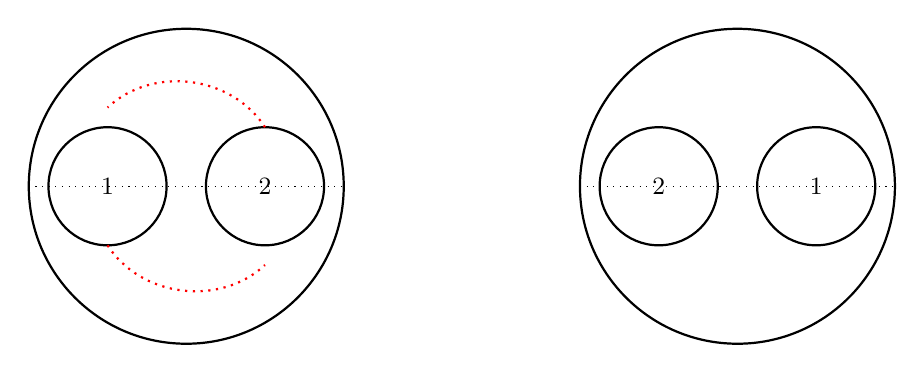
\begin{tikzpicture}
                        % basepoint
                        \node at (1, 0) {\small $2$};
                        \node at (-1, 0) {\small $1$};
                        
                        \draw[thick] (0,0) circle (2);
                        \draw[thick] (1, 0) circle (0.75);
                        \draw[thick] (-1, 0) circle (0.75);
                        \draw[dotted](-2, 0)--(2, 0);
                        \draw[thick, dotted, red] (-1, -0.75) to [bend right=50] (1, -1);
                        \draw[thick, dotted, red] (1, 0.75) to [bend right=50] (-1, 1);

                        \node at (3.5, 0) {$\rightsquigarrow$};
                        
                        % twisted basepoint
                        \node at (8, 0) {\small $1$};
                        \node at (6, 0) {\small $2$};
                        
                        \draw[thick] (7,0) circle (2);
                        \draw[thick] (8, 0) circle (0.75);
                        \draw[thick] (6, 0) circle (0.75);
                        \draw[dotted](5, 0)--(9, 0);  
                        
        \end{tikzpicture}
\end{center}

Since $\pi$ is an op-fibration, we obtain for a pair $(A,B)$ a cocartesian morphism 
$\beta' \colon (A,B) \to (B,A)$ in $\C^2$ with $\pi(\beta')=\beta$.

\end{const}

\begin{prop}
    Let $\B$ be a representable colored braided operad and $\C$ denoting its underlying category. Then the
    Construction \ref{con:braidmon} defines a braided monoidal structure on $\C$.
\end{prop}


% braided monoidal structure on a category $\C$
% that is induced by a op-fibration over the category $\Br$ also satisfying the Segal condition.
% To do so, we will need to choose paths of configurations in $\Br$ on various occasions.
% We will refrain from specifying the paths in detail but rather describe the paths enough to 
% understand from which homotopy class we choose a path so we then see why certain compositions 
% of paths are homotopy equivalent. Also, we do not care much about the size of the
% disks as we can expand and shrink them continuously as needed.
